
%\documentclass[aps,prl,twocolumn,showpacs,superscriptaddress,groupedaddress, floatfix]{revtex4-2}  % for review and submission
\documentclass[aps,preprint,showpacs,superscriptaddress,groupedaddress,linenumbers]{revtex4-2}  % for double-spaced preprint
\usepackage{graphicx}  % needed for figures
\usepackage{dcolumn}   % needed for some tables
\usepackage{bm}        % for math
\usepackage{amssymb}   % for math
\usepackage[caption=false]{subfig}

\begin{document}
\thispagestyle{empty}

{\normalsize \appendix{Appendix: Supplementary Material}\hfill\vspace*{4ex}}

\begin{figure*}[h]                         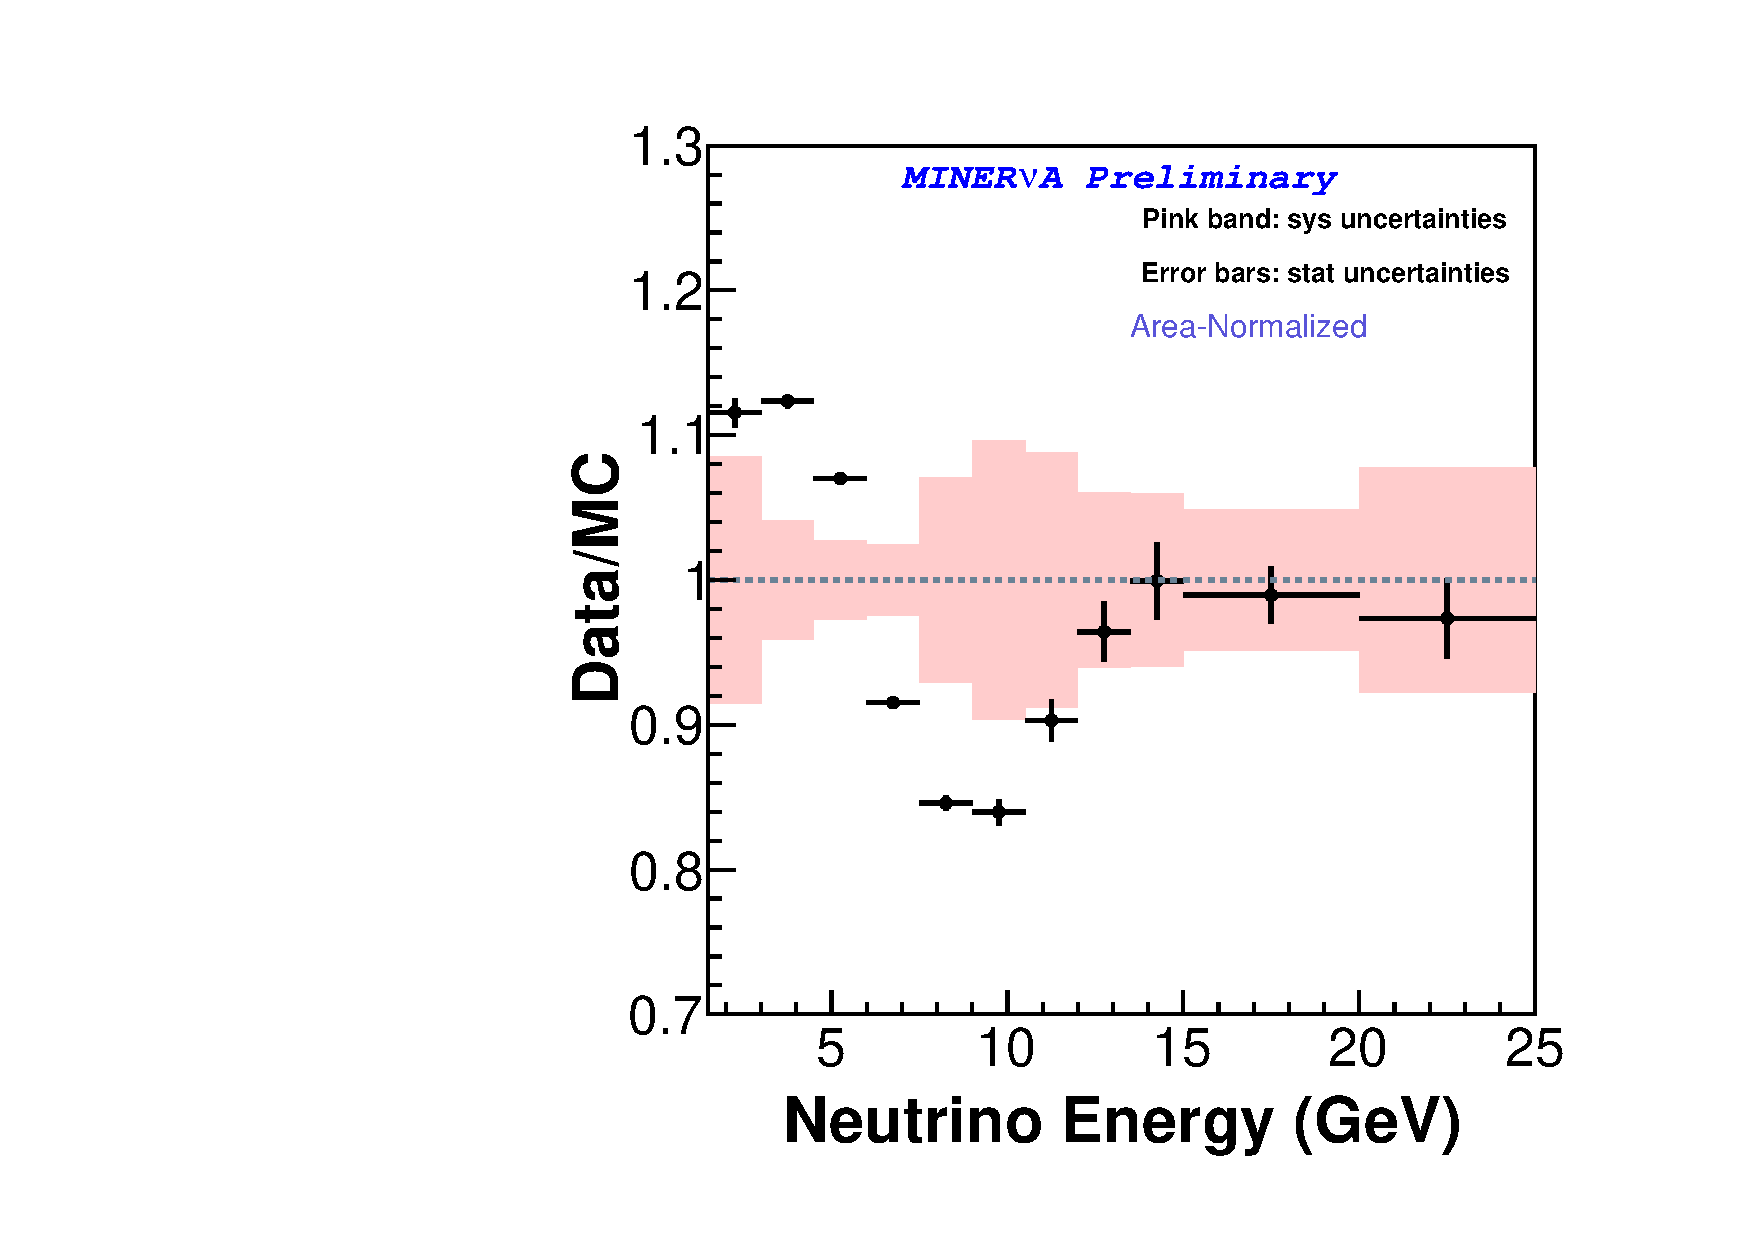
\includegraphics[width=.495\linewidth]{area_norm_data_nommc_ratio.pdf}
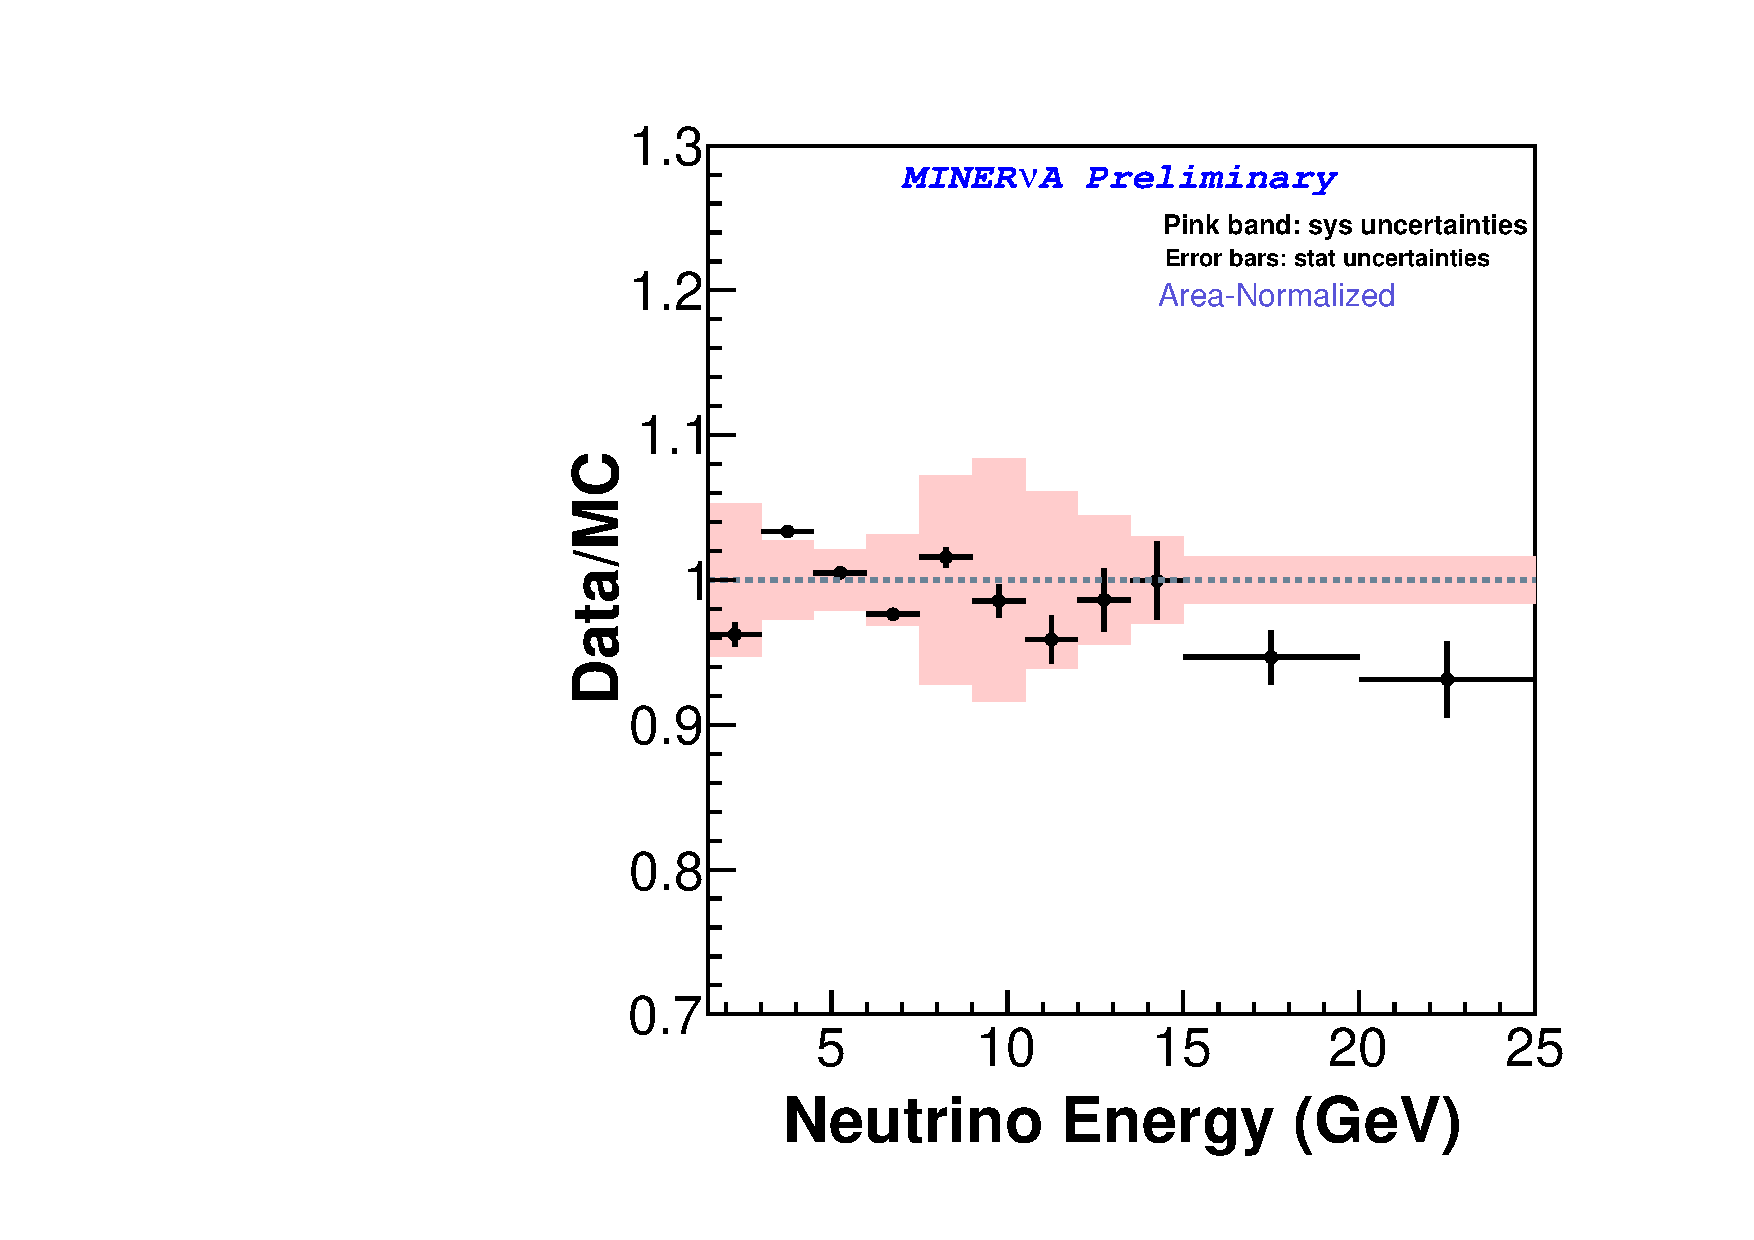
\includegraphics[width=.495\linewidth]{area_norm_data_rewgtmc_ratio.pdf}
    %\caption{Systematic 2D}
    \caption{Ratio of data to simulation as a function of reconstructed neutrino energy for events with less than 800~MeV of hadronic energy, before (left) and after (right) a fit which allowed flux and energy scale uncertainties to vary, as described in the body of the Letter.   The simulation has been normalized to the same number of events as the data. The black error bars correspond to the statistical uncertainty on the ratio and the pink band represents the shape component of the simulation's systematic uncertainty.  The ratio is shown for the first third of the POT collected but remained consistent throughout the entire run.     }
     \label{Sys2D} 
\end{figure*}

\begin{figure*}[h]  
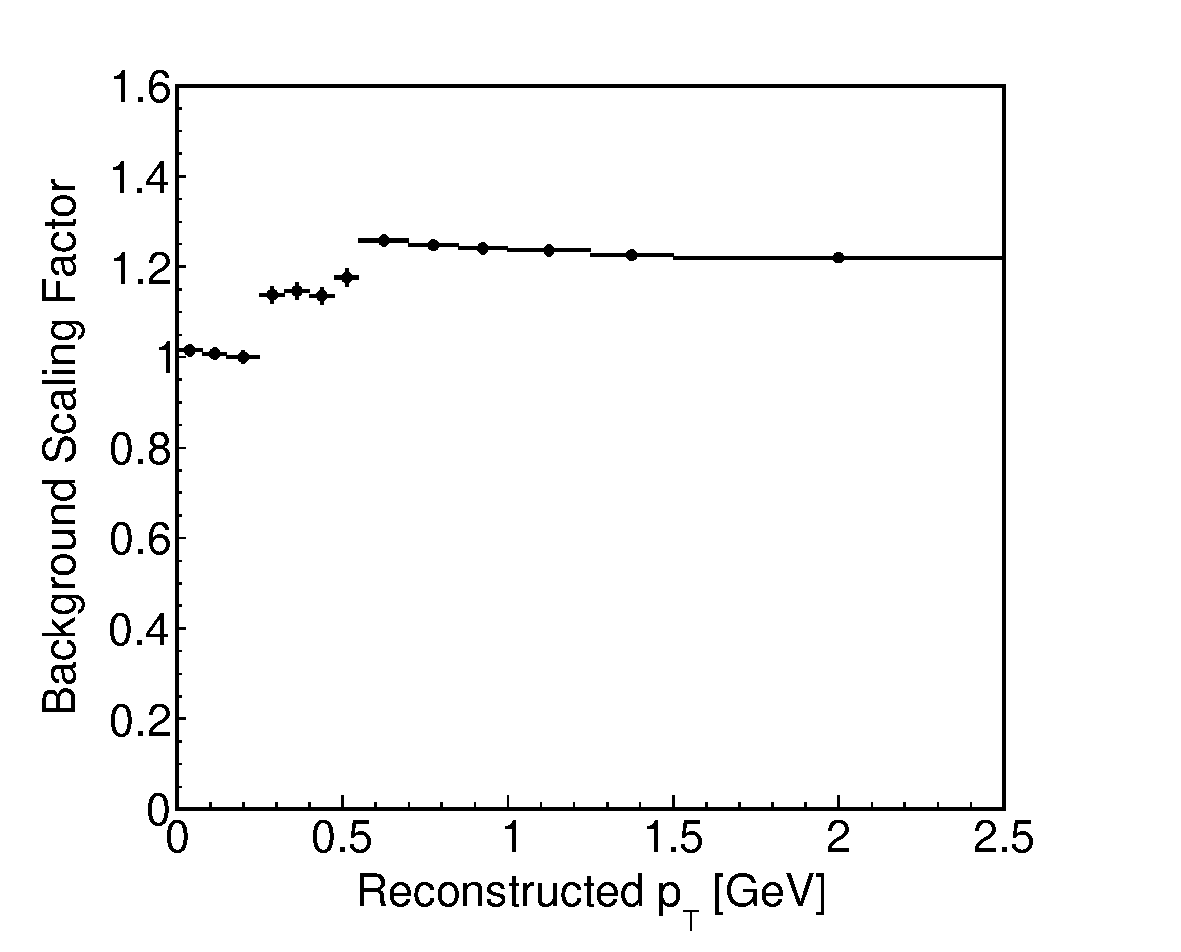
\includegraphics[width=.495\linewidth]{scalefactor_1track.pdf}
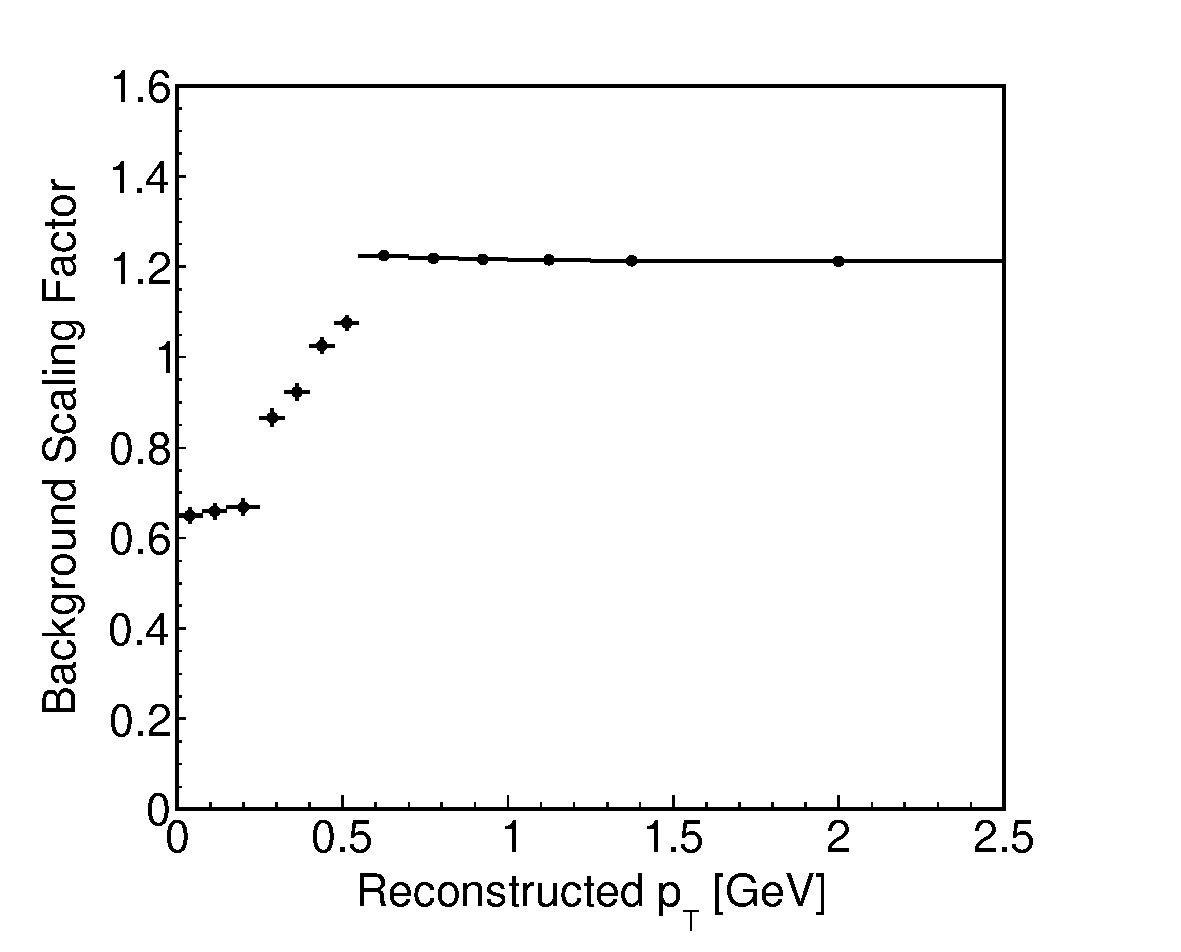
\includegraphics[width=.495\linewidth]{scalefactor_2track.pdf}
    %\caption{Systematic 2D}
    \caption{ Ratio of backgrounds versus reconstructed muon transverse momentum before and after the background fits described in the letter.      }
     \label{Sys2D} 
\end{figure*}

\begin{figure*}                         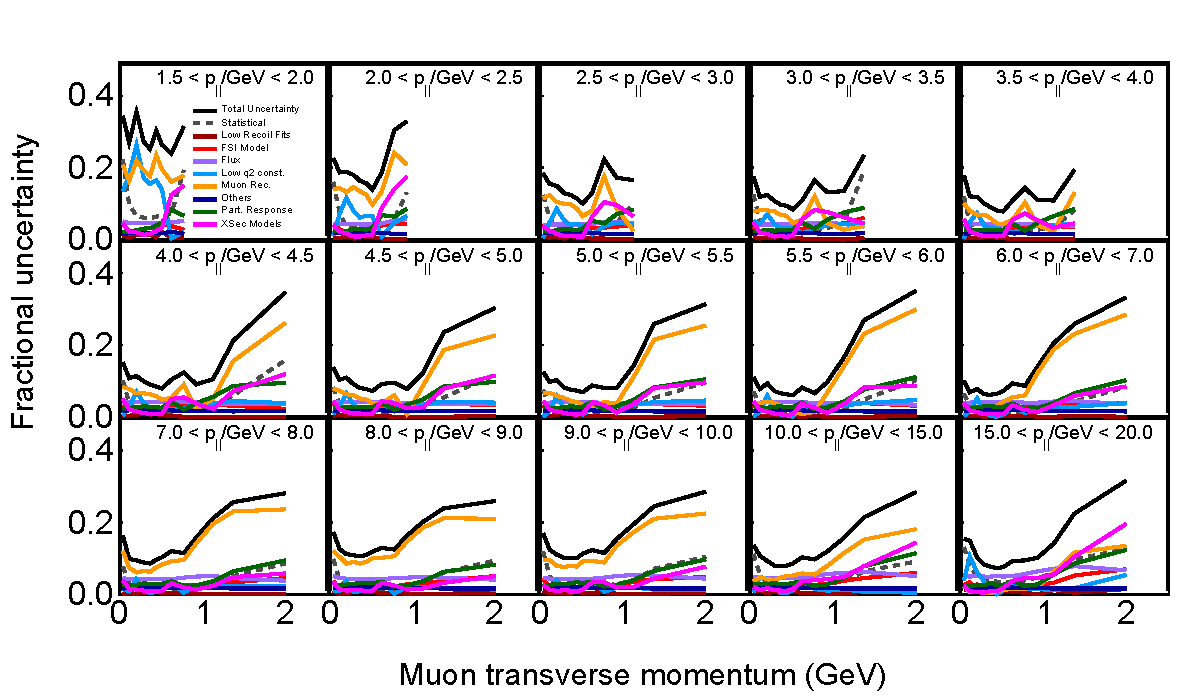
\includegraphics[width=\linewidth]{errors-pt.pdf}
    %\caption{Systematic 2D}
    \caption{Fractional systematic uncertainty on the double-differential cross section as a function of $p_\perp$ and $p_\parallel$.}
     \label{Sys2D} 
\end{figure*}


\begin{figure}                         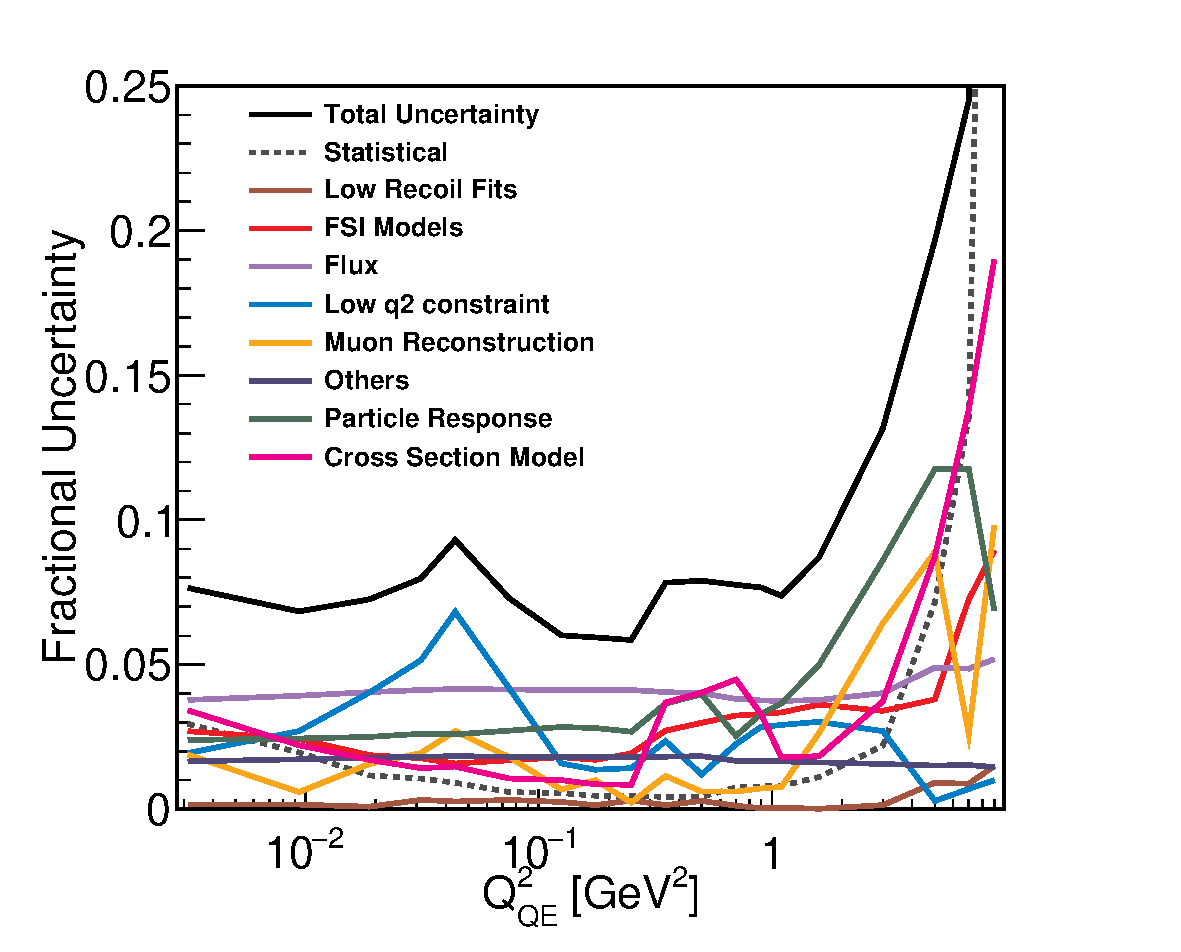
\includegraphics[trim={0cm 0cm 0cm 1.20cm},clip,width=\linewidth]{q2_log_errsum_nobck_unfold_effcor_cross_section_Feb2020.pdf}
    \caption{Fractional systematic uncertainty on the single-differential cross section as a function of $Q^2_{QE}$.}
     \label{Sys2D} 
\end{figure}

\begin{table}
\renewcommand*{\arraystretch}{1.2}
\begin{ruledtabular}
\begin{tabular}{lcc}

    &  $\chi^2$ &   $\chi^2$ \\ 
Model & Linear & Log \\
% \hline
% GENIE 2.12.6  &  444 & 539 \\
% \quad+RPA+$\pi$ tune &  141     &    241      \\ 
% \quad+RPA+$\pi$ tune+MINOS low $q^2$ sup. &   117      &    213     \\
% \hline
%  GENIE 2.12.6+ 2p2h &  1451  & 973 \\
% \quad+recoil fit+RPA+$\pi$ tune &   497     &  358 \\
% \quad+recoil fit+RPA+$\pi$ tune+MINOS low $q^2$ sup. & 240        &    208       \\
% \quad+recoil fit+$\pi$ tune &   1294          &   814      \\
% \quad+RPA+$\pi$ tune &   648     &   565      \\
% \hline
% NuWro LFG & & \\
% NuWro SF & & \\
% \hline
% GiBuu & & \\
\hline
GENIE 2.12.6 &	        292 &	        372 \\
%+recoil fit+RPA+$\pi$ tune &	        135 &	        242 \\
%\qquad+$\pi$ tune &	        322 &	        428 \\
\qquad+RPA+$\pi$ tune &	        135 &	        243 \\
\qquad+RPA+$\pi$ tune+MINOS $\pi$ low $Q^2$ sup. &	        120 &	        231 \\
\hline%+recoil fit+RPA+$\pi$ tune+Nieves low $Q^2$ sup. &	        131 &	        262 \\
%+recoil fit+$\pi$ tune &	        320 &	        428 \\
%+recoil fit + RPA + NonRES piontune + MINERvA $\pi$ tune low $Q^2$ sup. &	        147 &	        312 \\
GENIE 2.12.6 + 2p2h &	        909 &	        640 \\
\qquad+RPA+$\pi$ tune+recoil fit (MnvGENIEv1) &	        436 &	        344 \\
%\qquad+$\pi$ tune &	        961 &	        704 \\
\qquad+RPA+$\pi$ tune &	        442 &	        391 \\
\qquad+recoil fit+RPA+$\pi$ tune+MINOS $\pi$ low $Q^2$ sup. &	        216 &	        206 \\
%\qquad+recoil fit+RPA+$\pi$ tune+Nieves low $Q^2$ sup. &	        276 &	        241 \\
\qquad+recoil fit+$\pi$ tune &	       1019 &	        719 \\
\qquad+recoil fit+RPA+$\pi$ tune+MINERvA $\pi$ low $Q^2$ sup. (MnvGENIEv2) &	        199 &	        195 \\
%\qquad+RPA+$\pi$ tune &	        442 &	        391 \\
\hline
NuWro SF &	        498 &	        441 \\
NuWro LFG &	        363 &	        316 \\
\hline
GiBUU &	        353 &	        271 \\
%GENIE v3 &	        584 &	        257 \\

\end{tabular}
\end{ruledtabular}
\caption{\label{1DChi2} $\chi^2$ of various model variants compared to the differential cross section as a function of $Q^2$. Both standard and log-normal $\chi^2$ are shown, and the number of degrees of freedom for each comparison is 19.}
\end{table} 

\end{document}
